\documentclass[12pt,a4paper]{report}

\usepackage{graphicx} % Ajouté pour l'inclusion des images
\usepackage{float} % Ajouté pour l'option [H] dans les figures
\usepackage{hyperref} % Ajouté pour la commande \url




\begin{document}




% ----------------------
% PAGE DE GARDE
% ----------------------
\begin{titlepage}
    \centering
    %\vspace*{1cm}
    %
\includegraphics[width=0.25\textwidth]{Logo_ESPRIT_Ariana.jpg}
    %\vspace{1cm}
    {\Huge \textbf{Rapport de Stage} \par}
    \vspace{1.5cm}
    {\LARGE Développement d’un logiciel du chiffrage\par}
    \vspace{0.5cm}
    {\Large \textbf{eco-pilot} \par}
    \vspace{1cm}
    
\includegraphics[width=0.18\textwidth]{Logo_ESPRIT_Ariana.jpg}
    \vspace{2cm}
    \vfill
    \begin{flushright}
        \textbf{Stagiaire :} Mayar Briki \\
        \textbf{Encadrant académique :} Nom Prénom \\
        \textbf{Encadrant professionnel :} Nom Prénom \\
        \textbf{Date :} \today
    \end{flushright}
    % Logo parfaitement aligné à gauche en bas de page
    %\vspace{1cm}
    %\hspace*{0pt}
\includegraphics[width=0.18\textwidth]{Logo_ESPRIT_Ariana.jpg}
\end{titlepage}


% ----------------------
% INTRODUCTION
% ----------------------
\chapter{Introduction}
Durant mon stage de deux mois, j’ai eu l’opportunité de découvrir et de participer à des projets liés à la gestion de projets et à la gestion de budgets à travers un logiciel de chiffrage. Ce stage m’a permis de comprendre l’importance de l’organisation, du suivi des coûts et de l’optimisation des ressources pour assurer le succès des projets, tout en développant mes compétences pratiques dans un environnement professionnel. \textbf{eco-pilote}.  

% ----------------------
% PROJET
% ----------------------
\chapter{Présentation générale du projet }
\section{Contexte et objectifs}
Ce projet a été réalisé dans le cadre d’un stage de deux mois.  
\section{Utilisateurs cibles}
L’application s’adresse principalement aux professionnels impliqués dans la gestion de projets et le chiffrage budgétaire. Les utilisateurs cibles incluent :

\begin{itemize}
    \item \textbf{Chefs de projet :} responsables de la planification, du suivi et de la gestion des ressources et des coûts des projets.
    \item \textbf{Responsables financiers :} chargés de la validation des budgets, du contrôle des dépenses et de l’optimisation des coûts.
    \item \textbf{Membres d’équipes techniques :} intervenant dans la saisie des besoins, la consultation des articles et la remontée d’informations sur l’avancement des tâches.
    \item \textbf{Administrateurs :} assurant la gestion des utilisateurs, des droits d’accès et la configuration générale de l’application.
    \item \textbf{Clients ou partenaires externes :} pouvant accéder à certaines informations ou suivre l’avancement des projets selon les droits qui leur sont attribués.
\end{itemize}

Cette diversité d’utilisateurs implique une gestion fine des rôles et des permissions afin de garantir la sécurité et la pertinence des informations accessibles à chacun.
\section{Fonctionnalités principales}
Les principales fonctionnalités du projet incluent :
\begin{itemize}
    \item \textbf{Gestion des utilisateurs :} Création, modification, suppression et gestion des rôles des utilisateurs. Chaque utilisateur dispose d’un profil personnalisé avec des droits d’accès adaptés à sa fonction (administrateur, chef de projet, membre technique, etc.). Un système d’authentification sécurisé permet de garantir la confidentialité des données et la traçabilité des actions.
    \item \textbf{Gestion des articles :} Ajout, mise à jour, suppression et consultation des articles. Les articles représentent les ressources, matériaux ou prestations nécessaires à la réalisation des projets. Un catalogue centralisé facilite la recherche, la comparaison et la sélection des articles, tout en permettant la gestion des stocks et des coûts associés.
    \item \textbf{Gestion des projets :} Suivi, planification et gestion des différents projets. Cette fonctionnalité permet de créer de nouveaux projets, d’y associer des utilisateurs, des articles et des budgets, et de suivre l’avancement des tâches. Des outils de reporting et de visualisation (tableaux de bord, graphiques) aident à piloter efficacement les projets et à anticiper les dérives budgétaires ou organisationnelles.
\end{itemize}

% ----------------------
% CAHIER DES CHARGES
% ----------------------
\chapter{Cahier des charges}
\section{Besoins fonctionnels}
\section{Besoins techniques}
\section{Contraintes}

% ----------------------
% TECHNOLOGIES
% ----------------------
\chapter{Étude et choix technologiques}

Présentation du choix de la stack \textbf{PERN (PostgreSQL, Express, React, Node.js)} et justification.  

\begin{center}
    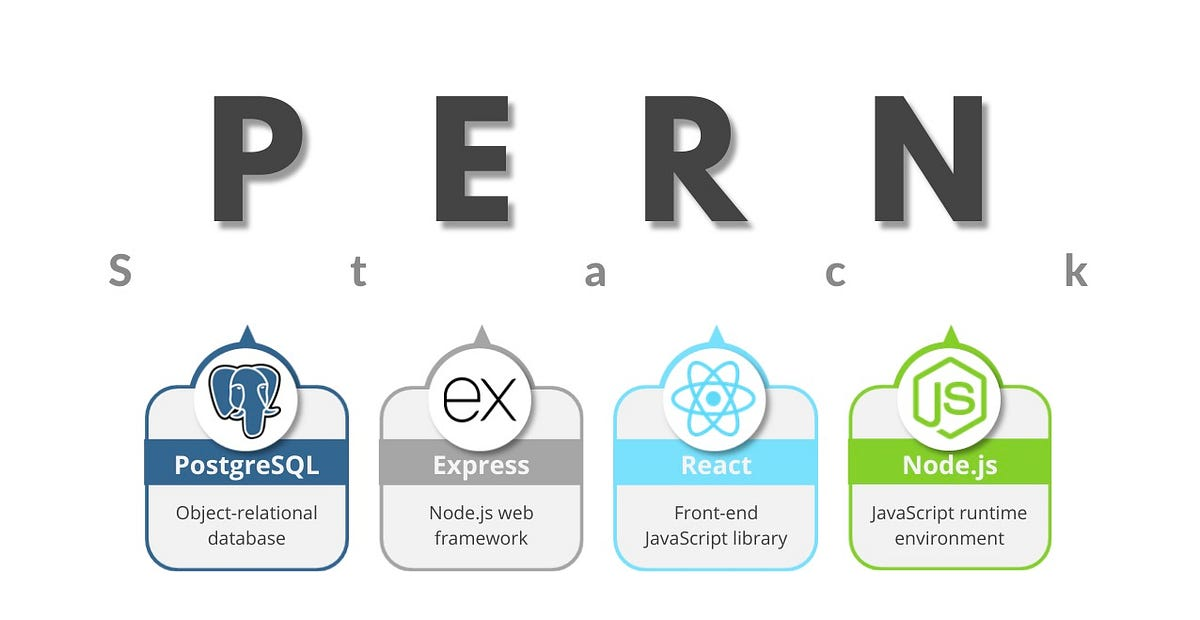
\includegraphics[width=0.4\textwidth]{1_ptqverAyBpdfUDhrs2g_3A.jpg} % Mets ton logo ici
\end{center}

\section*{Présentation détaillée de la stack PERN}

La stack \textbf{PERN} est composée de quatre technologies principales, chacune jouant un rôle spécifique dans l’architecture de l’application :

\begin{itemize}
    \item \textbf{PostgreSQL :} Système de gestion de base de données relationnelle open-source reconnu pour sa robustesse, sa conformité aux standards SQL et ses fonctionnalités avancées (transactions, gestion des relations complexes, extensibilité). Il permet de garantir l’intégrité et la sécurité des données, tout en offrant de bonnes performances pour des applications à grande échelle.
    \item \textbf{Express.js :} Framework minimaliste pour Node.js, Express simplifie la création d’API RESTful et la gestion des routes, des middlewares et des requêtes HTTP. Il favorise une architecture modulaire et maintenable, tout en restant léger et performant.
    \item \textbf{React :} Bibliothèque JavaScript développée par Facebook pour la création d’interfaces utilisateur dynamiques et réactives. React permet de construire des composants réutilisables, d’optimiser le rendu grâce au Virtual DOM et de gérer efficacement l’état de l’application côté client.
    \item \textbf{Node.js :} Environnement d’exécution JavaScript côté serveur, Node.js se distingue par son modèle événementiel non bloquant, idéal pour les applications nécessitant une forte scalabilité et un traitement asynchrone des requêtes.
\end{itemize}

\section*{Justification du choix de la stack PERN}

La stack \textbf{PERN} (PostgreSQL, Express, React, Node.js) a été choisie pour plusieurs raisons :  

\begin{itemize}
    \item \textbf{JavaScript full-stack :} Avec Node.js et React, le même langage est utilisé côté serveur et côté client, ce qui simplifie le développement et la maintenance.
    \item \textbf{Base de données relationnelle robuste :} PostgreSQL offre une gestion avancée des données, des relations complexes et une grande fiabilité pour les applications critiques.
    \item \textbf{Performance et scalabilité :} Node.js, grâce à son modèle non-bloquant et orienté événement, permet de gérer efficacement un grand nombre de requêtes simultanées.
    \item \textbf{Flexibilité et modularité :} Express.js facilite la création d’API RESTful flexibles, tandis que React permet de construire une interface utilisateur dynamique et réactive.
    \item \textbf{Écosystème riche :} Chaque composant de la stack dispose d’une communauté active et de nombreux packages, accélérant le développement et l’intégration de fonctionnalités avancées.
\end{itemize}

\section*{Comparaison avec d’autres stacks populaires}

Il existe d’autres stacks populaires telles que \textbf{MERN} (MongoDB, Express, React, Node.js) et \textbf{LAMP} (Linux, Apache, MySQL, PHP). Le choix de PERN s’explique par les avantages suivants :

\begin{itemize}
    \item \textbf{Par rapport à MERN :} PostgreSQL offre des fonctionnalités relationnelles avancées et une meilleure gestion des transactions que MongoDB, ce qui est crucial pour des applications nécessitant une forte cohérence des données.
    \item \textbf{Par rapport à LAMP :} La stack PERN permet un développement full JavaScript, réduisant la courbe d’apprentissage et facilitant la communication entre les différentes couches de l’application. De plus, Node.js offre de meilleures performances pour les applications temps réel.
    \item \textbf{Évolutivité et modernité :} La stack PERN est particulièrement adaptée aux applications web modernes nécessitant une interface utilisateur réactive et une API performante.
\end{itemize}

En résumé, la stack PERN combine la puissance d’une base de données relationnelle, la flexibilité du JavaScript full-stack et la modernité des outils de développement web actuels, ce qui en fait un choix pertinent pour le projet \textbf{eco-pilot}.

% ----------------------
% CONCEPTION
% ----------------------
\chapter{Conception du projet}
\section{Architecture de l’application}
Inclure un schéma de l’architecture PERN.  

\section{Diagrammes UML}

\begin{figure}[H]
    \centering
    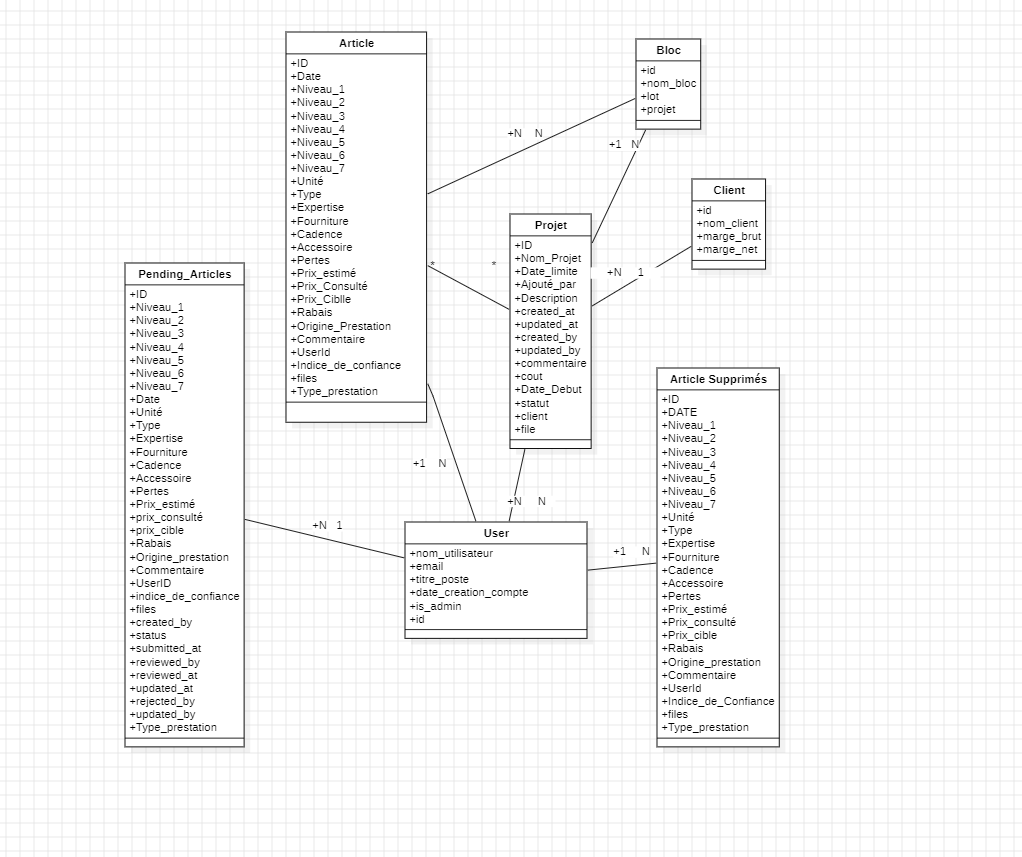
\includegraphics[width=0.5\linewidth]{image.png}
    \caption{Diagramme UML principal de l’application}
    \label{fig:placeholder}
\end{figure}

\textbf{Description du diagramme~:}

Le diagramme UML ci-dessus illustre l’architecture principale de l’application \textbf{eco-pilot}. On y distingue les entités essentielles et leurs relations :

\begin{itemize}
    \item \textbf{Utilisateur (User) :} Représente les différents profils accédant à l’application (administrateur, chef de projet, membre technique, etc.). Chaque utilisateur possède des attributs comme l’identifiant, le nom, l’email, le mot de passe (hashé) et un rôle.
    \item \textbf{Projet (Project) :} Entité centrale du système, chaque projet est associé à un ou plusieurs utilisateurs (gestion de l’équipe projet), à un budget, à des articles et à un état d’avancement.
    \item \textbf{Article :} Représente les ressources, matériaux ou prestations nécessaires à la réalisation des projets. Chaque article possède des informations telles que le nom, la description, le coût unitaire et le stock disponible.
    \item \textbf{Budget :} Associé à chaque projet, il permet de suivre les coûts prévus et réels, ainsi que les écarts éventuels.
    \item \textbf{Relations :} 
    \begin{itemize}
        \item Un utilisateur peut participer à plusieurs projets, et un projet peut avoir plusieurs utilisateurs (relation plusieurs-à-plusieurs).
        \item Un projet peut contenir plusieurs articles, chaque article pouvant être utilisé dans plusieurs projets (relation plusieurs-à-plusieurs).
        \item Chaque projet dispose d’un budget unique, mais le modèle peut être étendu pour gérer des budgets intermédiaires ou par lot.
    \end{itemize}
\end{itemize}

Ce diagramme met en évidence la structure relationnelle de l’application et sert de base à la conception de la base de données et des API.
\section{Modèle de la base de données}

% ----------------------
% IMPLÉMENTATION
% ----------------------
\chapter{Implémentation}
\section{Backend (Node.js + Express)}
\section{Frontend (React)}
\section{Base de données (MongoDB)}
\section{Sécurité et authentification (JWT, hashage)}
\section{Tests et validation}

% ----------------------
% DÉPLOIEMENT
% ----------------------
\chapter{Déploiement}
\section{Environnement de développement}

Le développement s’est effectué localement sur des machines équipées de Node.js, npm et PostgreSQL. Le code source est versionné avec Git et organisé en deux répertoires principaux : \texttt{client} (React) et \texttt{server} (Node.js/Express). Les variables d’environnement sont gérées via des fichiers \texttt{.env} pour séparer les configurations locales et de production.

\section{Environnement de production}

Pour le déploiement de l’application, deux plateformes cloud distinctes ont été utilisées afin de séparer le frontend et le backend :

\begin{itemize}
    \item \textbf{Frontend (React) :} Déployé sur \textbf{Vercel}, une plateforme spécialisée dans l’hébergement d’applications front-end modernes. Vercel offre un déploiement continu à partir du dépôt GitHub, une gestion automatique des builds, un CDN performant et des URLs de prévisualisation pour chaque branche ou pull request. Cela permet de garantir une mise en ligne rapide et fiable de l’interface utilisateur.
    \item \textbf{Backend (Node.js/Express) :} Hébergé sur \textbf{Render}, un service cloud qui facilite le déploiement d’API Node.js. Render gère automatiquement le scaling, la surveillance, les redémarrages en cas de panne et l’intégration continue. La connexion à la base de données PostgreSQL est également configurée sur Render, assurant la sécurité et la disponibilité des données.
\end{itemize}

La communication entre le frontend (Vercel) et le backend (Render) se fait via des appels API sécurisés (HTTPS). Les variables d’environnement de production sont configurées directement sur les tableaux de bord Vercel et Render pour garantir la confidentialité des clés et des accès.

\section{Gestion de versions (Git/GitHub)}
% ...existing code...

\section{CI/CD (si applicable)}
% ...existing code...

% ----------------------
% RÉSULTATS
% ----------------------
\chapter{Résultats obtenus}
Inclure captures d’écran de l’application (ex. page de connexion, tableau de bord).  

% ----------------------
% DIFFICULTÉS ET SOLUTIONS
% ----------------------
\chapter{Difficultés rencontrées et solutions}
Lister les problèmes techniques et organisationnels rencontrés ainsi que leurs solutions.  

% ----------------------
% PERSPECTIVES
% ----------------------
\chapter{Perspectives d’amélioration}
Améliorations techniques et fonctionnelles possibles.  

% ----------------------
% CONCLUSION
% ----------------------
\chapter{Conclusion}
Bilan global du stage, apports professionnels et personnels.  

% ----------------------
% ANNEXES
% ----------------------
\appendix
\chapter{Annexes}
\section{Extraits de code}
\section{Documentation API}
\section{Diagrammes complets}

% ----------------------
% BIBLIOGRAPHIE
% ----------------------
\begin{thebibliography}{9}
\bibitem{mern} Documentation officielle MERN : \url{https://www.mongodb.com/mern-stack}
\bibitem{react} Documentation React : \url{https://react.dev}
\bibitem{node} Documentation Node.js : \url{https://nodejs.org}
\end{thebibliography}

\end{document}


\section{Introduction}


\end{document}
